\documentclass[tikz]{standalone}
\usetikzlibrary{calc, intersections, math}

\begin{document}
	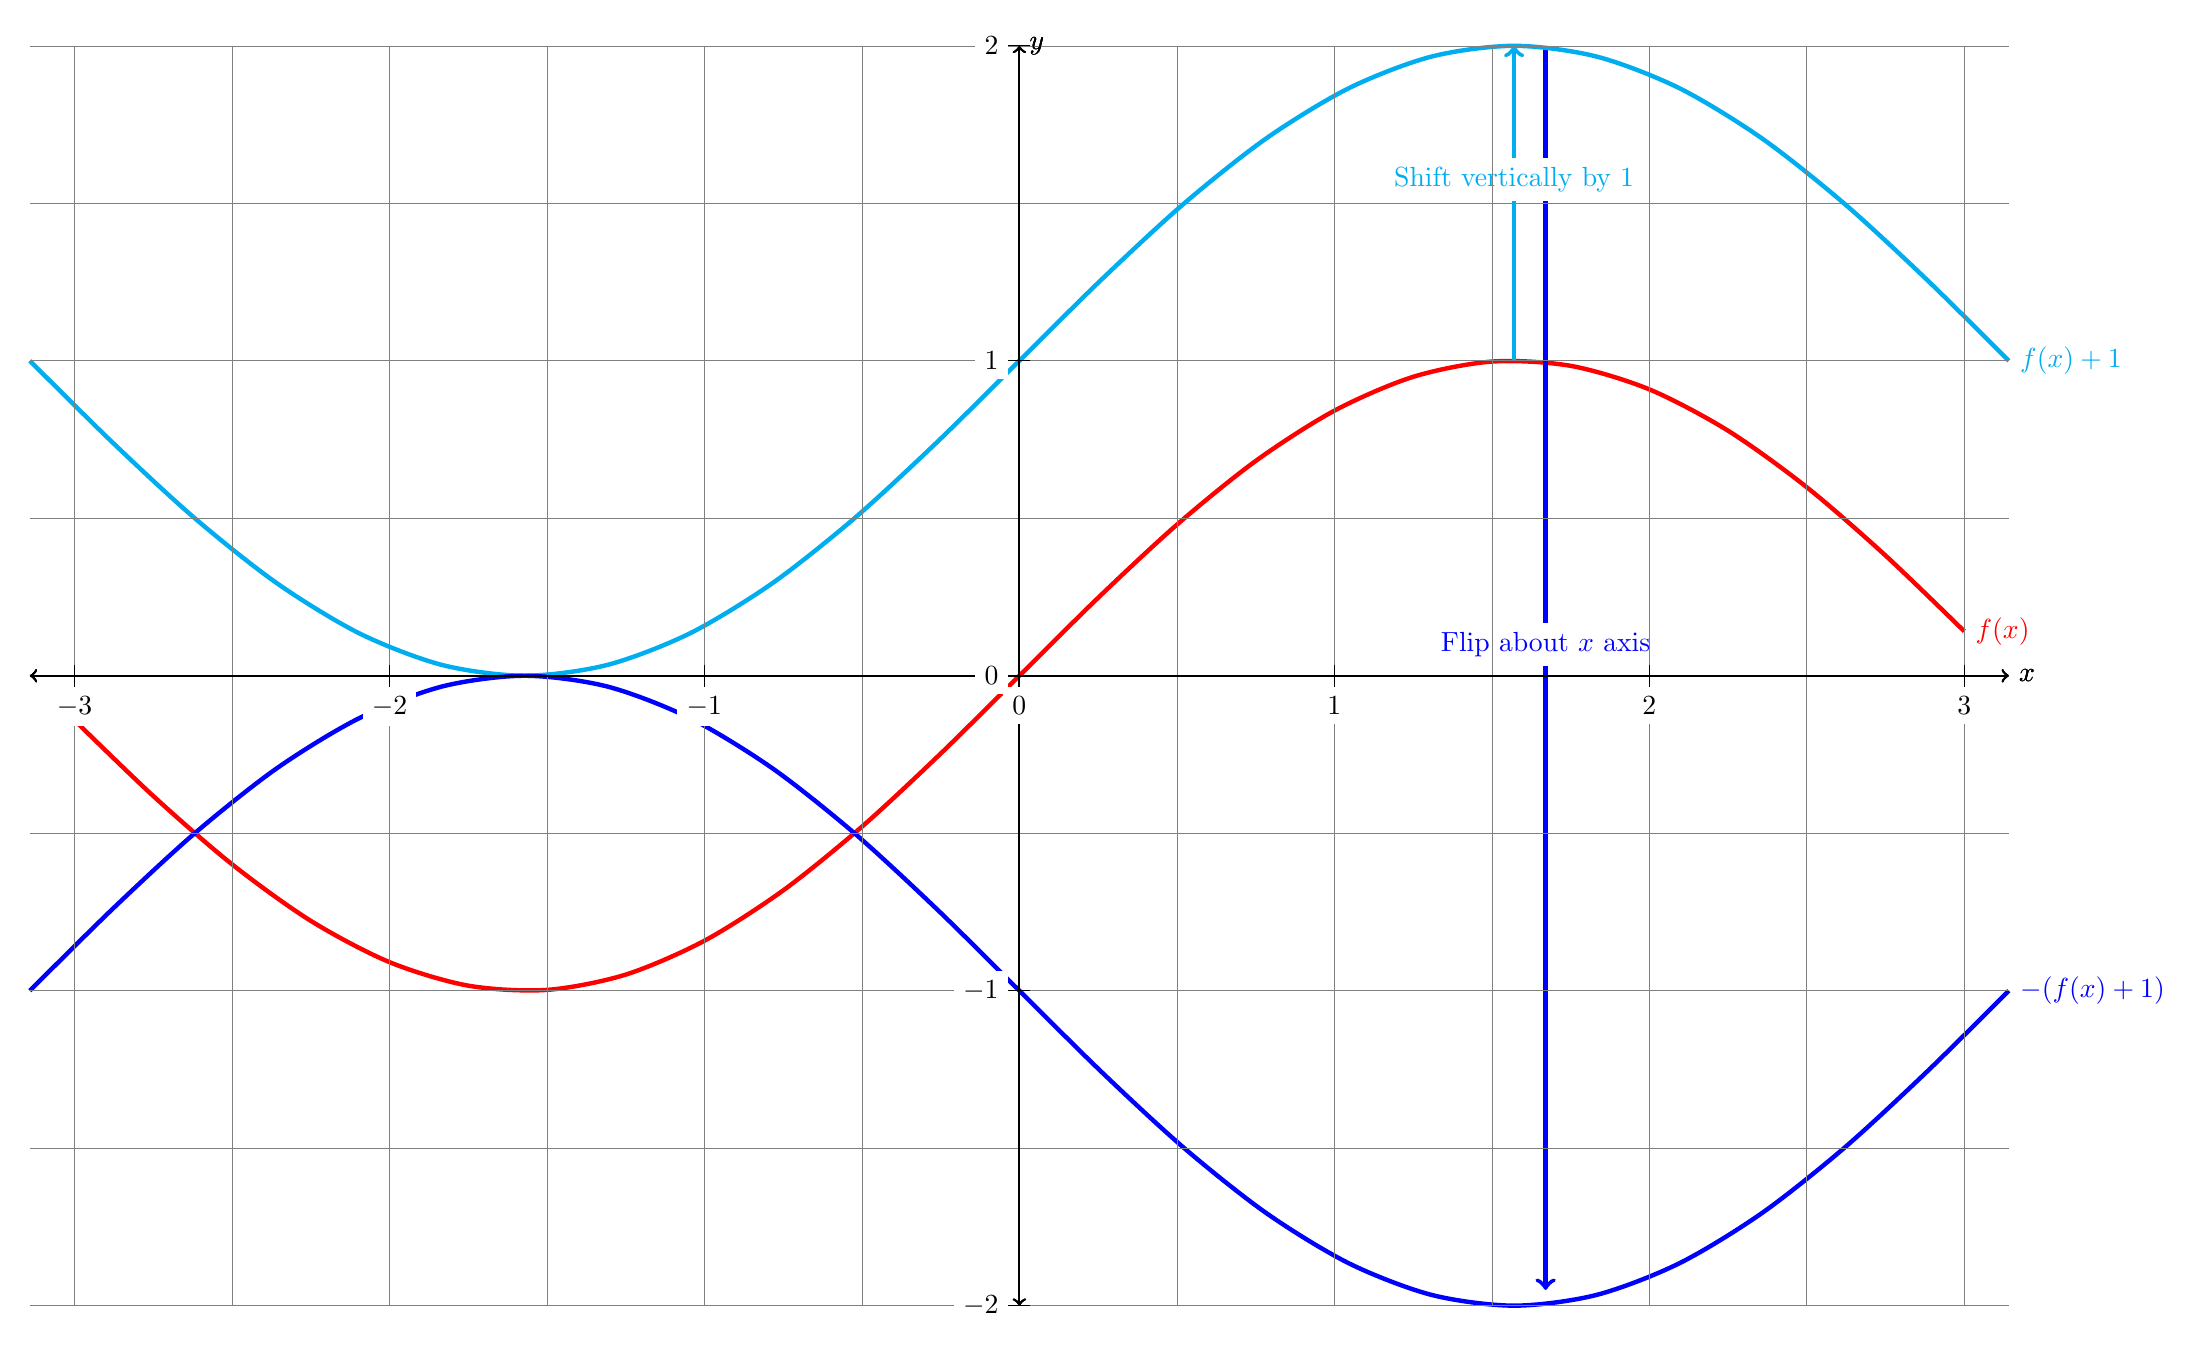
\begin{tikzpicture}[scale=4, mystyle/.style={circle,fill}]


	\draw[ultra thick,red,domain=-3:3,smooth] plot (\x,{sin(\x r)}) node[right] {$f(x)$};

	\draw[ultra thick, blue, ->] (pi/2+.1,2) -- (pi/2+.1,-1.95) node[midway, above, fill=white] {Flip about $x$ axis};
	\draw[ultra thick, cyan, ->] (pi/2,1) -- (pi/2,2) node[midway, above, fill=white] {Shift vertically by $1$};



	\draw[ultra thick,cyan,domain=-pi:pi,smooth] plot (\x,{sin(\x r)+1}) node[right] {$f(x)+1$};
	\draw[ultra thick,blue,domain=-pi:pi,smooth] plot (\x,{-1*sin(\x r)-1}) node[right] {$-(f(x)+1)$};

	% this file contains the background (axes, tickmarks, etc) for the graph translation plots. Import it using % this file contains the background (axes, tickmarks, etc) for the graph translation plots. Import it using % this file contains the background (axes, tickmarks, etc) for the graph translation plots. Import it using \input{fig-Graph-Translations-Background.tex} in the body of the tikz figure

% set the window size. The \c notation allows us to use more complex variable names
\tikzmath{\c{width} = pi;}

% setting up the Cartesian Grid. Note "help lines" = "gray, very thin"
\draw[step=.5cm,help lines] (-1*\c{width},-2) grid (\c{width},2);
% setting up the real and imaginary axis. 
\draw[thick, <->] (-1*\c{width},0) -- (\c{width},0) coordinate (x axis) node[right] {$x$};
\draw[thick, <->] (0,-2) -- (0,2) coordinate (y axis) node[right] {$y$};;

\foreach \x in {-3,-2, ..., 3}
	\draw (\x cm,1pt) -- (\x cm,-1pt) node[anchor=north, fill=white] {$\x$};
\foreach \y in {-2,-1,0,1,2}
	\draw (1pt,\y cm) -- (-1pt,\y cm) node[anchor=east, fill=white] {$\y$};
 in the body of the tikz figure

% set the window size. The \c notation allows us to use more complex variable names
\tikzmath{\c{width} = pi;}

% setting up the Cartesian Grid. Note "help lines" = "gray, very thin"
\draw[step=.5cm,help lines] (-1*\c{width},-2) grid (\c{width},2);
% setting up the real and imaginary axis. 
\draw[thick, <->] (-1*\c{width},0) -- (\c{width},0) coordinate (x axis) node[right] {$x$};
\draw[thick, <->] (0,-2) -- (0,2) coordinate (y axis) node[right] {$y$};;

\foreach \x in {-3,-2, ..., 3}
	\draw (\x cm,1pt) -- (\x cm,-1pt) node[anchor=north, fill=white] {$\x$};
\foreach \y in {-2,-1,0,1,2}
	\draw (1pt,\y cm) -- (-1pt,\y cm) node[anchor=east, fill=white] {$\y$};
 in the body of the tikz figure

% set the window size. The \c notation allows us to use more complex variable names
\tikzmath{\c{width} = pi;}

% setting up the Cartesian Grid. Note "help lines" = "gray, very thin"
\draw[step=.5cm,help lines] (-1*\c{width},-2) grid (\c{width},2);
% setting up the real and imaginary axis. 
\draw[thick, <->] (-1*\c{width},0) -- (\c{width},0) coordinate (x axis) node[right] {$x$};
\draw[thick, <->] (0,-2) -- (0,2) coordinate (y axis) node[right] {$y$};;

\foreach \x in {-3,-2, ..., 3}
	\draw (\x cm,1pt) -- (\x cm,-1pt) node[anchor=north, fill=white] {$\x$};
\foreach \y in {-2,-1,0,1,2}
	\draw (1pt,\y cm) -- (-1pt,\y cm) node[anchor=east, fill=white] {$\y$};


	\end{tikzpicture}


\end{document}
